\documentclass[handout, aspectratio=169]{beamer}

\usetheme{Warsaw}

\usepackage[brazil]{babel}
\usepackage[utf8]{inputenc}
\usepackage[T1]{fontenc}
\usepackage{times}
\usepackage{epsfig}
\usepackage{listings}
\usepackage{amsfonts}
\usepackage{multirow}
\usepackage{tikz}
\usepackage{textpos}

%\usepackage{dcolumn}
%\newcolumntype{.}{D{.}{.}{-1}}
%\newcolumntype{d}[1]{D{.}{.}{#1}}
%\usetheme{Berkeley}

\newcommand{\be}{\begin{enumerate}[<+->]}
\newcommand{\ee}{\end{enumerate}}
\newcommand{\bq}{\begin{quote}}
\newcommand{\eq}{\end{quote}}
\newcommand{\bd}{\begin{description}[<+->]}
\newcommand{\ed}{\end{description}}
\newcommand{\bi}{\begin{itemize}[<+->]}
\newcommand{\ei}{\end{itemize}}

\title[Linguagens de Programação]
{%
	Introdução%
}
\author[Prof. Hugo de Paula]
{
	Prof.~Hugo~de~Paula
}
\institute[DCC / PUC Minas]
{
\epsfig{file=puclogo_small_bw,width=1.5cm} \\
  \textsc{Pontifícia Universidade Católica de Minas Gerais}\\
	Departamento de Ciência da Computação
}
\date[]{}

\lstset{language=Java,
        basicstyle=\scriptsize,
        commentstyle=\color{red},
        showstringspaces=false,
        numbers=left,
        numberstyle=\tiny}

\begin{document}


\selectlanguage{brazil}

\begin{frame}
   \titlepage
\end{frame}

%\addtobeamertemplate{frametitle}{}{%
%	\begin{tikzpicture}[remember picture,overlay]
%	\node[anchor=north east,yshift=2pt] at (current page.north east) {
\epsfig{file=puclogo_small_bw,width=1.2cm}};
%	\end{tikzpicture}}


%\addtobeamertemplate{frametitle}{}{%
	%\begin{tikzpicture}[node distance=0cm, remember picture, overlay, every node/.style={inner sep=0,outer sep=0, node distance=0cm, baseline=0cm}]
	%\node[anchor=north east] at (current page.north east) {
\epsfig{file=puclogo_small_bw,width=1cm}};
	%\end{tikzpicture}}


%\logo{
\includegraphics[height=0.8cm]{puclogo_small_bw.pdf}\vspace{220pt}}


\begin{frame}
   \frametitle{Sumário}
   \tableofcontents[pausesections]
\end{frame}

%\AtBeginSection[] % Do nothing for \section*
%{
%\begin{frame}<beamer>
%\frametitle{Outline}
%\tableofcontents[currentsection]
%\end{frame}}


\addtobeamertemplate{frametitle}{}{%
   \begin{textblock*}{10mm}(.9945\textwidth,-2.02cm)
	   
\includegraphics[height=1cm]{puclogo_small_bw.pdf}
   \end{textblock*}
}



\section{Introdução}

\subsection{Linguagens de Programação}

\begin{frame}{Linguagens de programação}
   \bi
   \item ``É qualquer notação para a descrição de algoritmos e estruturas de dados'' \\ (\textit{\scriptsize  Pratt, 1975. Programming Languages: Design and Implementation}). \\[5mm]
   \item ``Uma linguagem que tem por objetivo expressar programas de computador e é capaz de expressar qualquer programa de computador'' \\ (\textit{\scriptsize MacLennan, 2016. Principles of Programming Languages: Design, Evaluation, and Implementation}).
   \ei
\end{frame}

\subsection{Nível de abstração}


\begin{frame}{Abstração}
   \bi
   \item A abstração permite a distinção entre categorias e indivíduos, ou classes e instâncias.
	\item Por exemplo: Um carro, do nível mais abstrato para o mais concreto:
		\bi
		\item um veículo automotor (pode ser moto, caminhão, caro, etc...)
        \item um carro propriamente dito
        \item um carro de passeio ou uma SUV
        \item um Koenigsegg CC
        \item um Koenigsegg CC 2003
        \item um Koenigsegg CC 2003 do Geraldo
        \item um Koenigsegg CC 2003 do Geraldo no momento em que foi comprado
		\ei
  \ei
\end{frame}

\begin{frame}{Abstração}


\begin{block}{Nível de abstração da linguagem}
\scriptsize
\centering
% \usepackage{tikz}
% The following commands are not supported in PSTricks at present
% We define them conditionally, so when they are implemented,
% this pgf file will use them.
\ifx\du\undefined
  \newlength{\du}
\fi
\setlength{\du}{15\unitlength}
\begin{tikzpicture}
\pgftransformxscale{0.600000}
\pgftransformyscale{-0.600000}
\definecolor{dialineblack}{rgb}{0.0, 0.0, 0.0}
\definecolor{dialinewhite}{rgb}{1.0, 1.0, 1.0}
\definecolor{dialinegray}{rgb}{0.501961, 0.501961, 0.501961}
\pgfsetstrokecolor{dialineblack}
\pgfsetfillcolor{dialinewhite}
\pgfsetlinewidth{0.100000\du}
\pgfsetdash{}{0pt}

%Desenha o bonequinho
\pgfpathellipse{\pgfpoint{7.950000\du}{2.650000\du}}{\pgfpoint{0.300000\du}{0\du}}{\pgfpoint{0\du}{0.300000\du}}
\pgfusepath{fill}
\pgfpathellipse{\pgfpoint{7.950000\du}{2.650000\du}}{\pgfpoint{0.300000\du}{0\du}}{\pgfpoint{0\du}{0.300000\du}}
\pgfusepath{stroke}
\draw (6.750000\du,3.250000\du)--(9.150000\du,3.250000\du);
\draw (7.950000\du,2.950000\du)--(7.950000\du,4.450000\du);
\draw (7.950000\du,4.450000\du)--(6.750000\du,5.750000\du);
\draw (7.950000\du,4.450000\du)--(9.150000\du,5.750000\du);
\node at (7.950000\du,6.990000\du){Desenvolvedor};

%Desenha o computador
\pgfsetfillcolor{dialineblack}
\fill (6.894444\du,15.800000\du)--(9.005556\du,15.800000\du)--(9.005556\du,17.022222\du)--(9.450000\du,17.800000\du)--(6.450000\du,17.800000\du)--(6.894444\du,17.022222\du)--cycle;
\pgfsetstrokecolor{dialineblack}
\draw (6.894444\du,15.800000\du)--(9.005556\du,15.800000\du)--(9.005556\du,17.022222\du)--(9.450000\du,17.800000\du)--(6.450000\du,17.800000\du)--(6.894444\du,17.022222\du)--cycle;
\pgfsetlinewidth{0.010000\du}
\pgfsetbuttcap
\pgfsetmiterjoin
\pgfsetdash{}{0pt}
\pgfsetstrokecolor{dialinewhite}
\draw (6.894444\du,15.800000\du)--(9.005556\du,15.800000\du)--(9.005556\du,17.022222\du)--(9.450000\du,17.800000\du)--(6.450000\du,17.800000\du)--(6.894444\du,17.022222\du)--cycle;
\pgfsetbuttcap
\pgfsetmiterjoin
\pgfsetdash{}{0pt}
\definecolor{dialinecolor}{rgb}{0.501961, 0.501961, 0.501961}
\pgfsetstrokecolor{dialinecolor}
\draw (6.894444\du,17.022222\du)--(9.005556\du,17.022222\du);
\pgfsetlinewidth{0.100000\du}
\pgfsetbuttcap
\pgfsetmiterjoin
\pgfsetdash{}{0pt}
\definecolor{dialinecolor}{rgb}{1.000000, 1.000000, 1.000000}
\pgfsetfillcolor{dialinecolor}
\fill (6.950000\du,15.855556\du)--(8.950000\du,15.855556\du)--(8.950000\du,16.966667\du)--(6.950000\du,16.966667\du)--cycle;
\definecolor{dialinecolor}{rgb}{0.000000, 0.000000, 0.000000}
\pgfsetstrokecolor{dialinecolor}
\draw (6.950000\du,15.855556\du)--(8.950000\du,15.855556\du)--(8.950000\du,16.966667\du)--(6.950000\du,16.966667\du)--cycle;
\pgfsetlinewidth{0.010000\du}
\pgfsetbuttcap
\pgfsetmiterjoin
\pgfsetdash{}{0pt}
\definecolor{dialinecolor}{rgb}{0.000000, 0.000000, 0.000000}
\pgfsetstrokecolor{dialinecolor}
\draw (6.950000\du,15.855556\du)--(8.950000\du,15.855556\du)--(8.950000\du,16.966667\du)--(6.950000\du,16.966667\du)--cycle;
\pgfsetbuttcap
\pgfsetmiterjoin
\pgfsetdash{}{0pt}
\definecolor{dialinecolor}{rgb}{1.000000, 1.000000, 1.000000}
\pgfsetstrokecolor{dialinecolor}
\draw (6.866667\du,17.272222\du)--(9.033333\du,17.272222\du);
\pgfsetbuttcap
\pgfsetmiterjoin
\pgfsetdash{}{0pt}
\definecolor{dialinecolor}{rgb}{1.000000, 1.000000, 1.000000}
\pgfsetstrokecolor{dialinecolor}
\draw (6.825000\du,17.341667\du)--(9.075000\du,17.341667\du);
\pgfsetbuttcap
\pgfsetmiterjoin
\pgfsetdash{}{0pt}
\definecolor{dialinecolor}{rgb}{1.000000, 1.000000, 1.000000}
\pgfsetstrokecolor{dialinecolor}
\draw (6.908333\du,17.202778\du)--(8.991667\du,17.202778\du);
\pgfsetbuttcap
\pgfsetmiterjoin
\pgfsetdash{}{0pt}
\definecolor{dialinecolor}{rgb}{1.000000, 1.000000, 1.000000}
\pgfsetstrokecolor{dialinecolor}
\draw (6.783333\du,17.411111\du)--(6.950000\du,17.133333\du);
\pgfsetbuttcap
\pgfsetmiterjoin
\pgfsetdash{}{0pt}
\definecolor{dialinecolor}{rgb}{1.000000, 1.000000, 1.000000}
\pgfsetstrokecolor{dialinecolor}
\draw (9.116667\du,17.411111\du)--(8.950000\du,17.133333\du);
\pgfsetbuttcap
\pgfsetmiterjoin
\pgfsetdash{}{0pt}
\definecolor{dialinecolor}{rgb}{1.000000, 1.000000, 1.000000}
\pgfsetstrokecolor{dialinecolor}
\draw (6.783333\du,17.411111\du)--(9.116667\du,17.411111\du);
\pgfsetbuttcap
\pgfsetmiterjoin
\pgfsetdash{}{0pt}
\definecolor{dialinecolor}{rgb}{1.000000, 1.000000, 1.000000}
\pgfsetstrokecolor{dialinecolor}
\draw (6.950000\du,17.133333\du)--(8.950000\du,17.133333\du);
\pgfsetbuttcap
\pgfsetmiterjoin
\pgfsetdash{}{0pt}
\definecolor{dialinecolor}{rgb}{1.000000, 1.000000, 1.000000}
\pgfsetstrokecolor{dialinecolor}
\draw (7.366667\du,17.411111\du)--(7.387500\du,17.341667\du);
\pgfsetbuttcap
\pgfsetmiterjoin
\pgfsetdash{}{0pt}
\definecolor{dialinecolor}{rgb}{1.000000, 1.000000, 1.000000}
\pgfsetstrokecolor{dialinecolor}
\draw (8.512078\du,17.341671\du)--(8.512500\du,17.341667\du);
\pgfsetbuttcap
\pgfsetmiterjoin
\pgfsetdash{}{0pt}
\definecolor{dialinecolor}{rgb}{1.000000, 1.000000, 1.000000}
\pgfsetstrokecolor{dialinecolor}
\draw (8.533333\du,17.411111\du)--(8.512078\du,17.341671\du);
\pgfsetbuttcap
\pgfsetmiterjoin
\pgfsetdash{{1.000000\du}{1.000000\du}}{0\du}
\pgfsetdash{{0.200000\du}{0.200000\du}}{0\du}
\definecolor{dialinecolor}{rgb}{1.000000, 1.000000, 1.000000}
\pgfsetstrokecolor{dialinecolor}
\draw (7.783333\du,17.522222\du)--(8.116667\du,17.522222\du)--(8.172222\du,17.688889\du)--(7.727778\du,17.688889\du)--cycle;
% Mouse pad
\draw (7.783333\du,17.522222\du)--(8.116667\du,17.522222\du)--(8.172222\du,17.688889\du)--(7.727778\du,17.688889\du)--cycle;
\pgfsetbuttcap
{
\pgfsetdash{}{0pt}
\pgfsetfillcolor{dialineblack}
\pgfsetstrokecolor{dialineblack}
\draw (7.950000\du,7.50000\du)--(7.950000\du,15.800000\du);
}
\node[anchor=west] at (11.0    \du,2.0    \du){Linguagem};
\node[anchor=west] at (11.0    \du,2.800000\du){Natural};
\node[anchor=west] at (11.0    \du,17.0    \du){Linguagem};
\node[anchor=west] at (11.0    \du,17.800000\du){de Máquina};
\node[anchor=west] at (0.0    \du,2.0    \du){Alto nível};
\node[anchor=west] at (0.0    \du,2.800000\du){de abstração};
\node[anchor=west] at (0.0    \du,17.0    \du){Baixo nível};
\node[anchor=west] at (0.0    \du,17.800000\du){de abstração};
\node[anchor=west] at (0.0    \du,12.5    \du){Linguagem};
\node[anchor=west] at (0.0    \du,13.300000\du){Assembly};
\node[anchor=west] at (0.0    \du,9.0    \du){Linguagem};
\node[anchor=west] at (0.0    \du,9.800000\du){de Programação};
\pgfsetbuttcap
{
\pgfsetlinewidth{0.100000\du}
\pgfsetdash{{\pgflinewidth}{0.200000\du}}{0cm}
\pgfsetdash{{\pgflinewidth}{0.200000\du}}{0cm}
\pgfsetarrowsend{stealth}
\draw (3.0    \du,8.0    \du)--(3.0    \du,4.0    \du);
\draw (3.0    \du,14.0    \du)--(3.0    \du,16.0    \du);
}
\end{tikzpicture}

\end{block}
\end{frame}




\begin{frame}{Domínios de programação}

\begin{itemize}
    \item Aplicações científicas
    \begin{itemize}
    \item Grande quantidade de operações de ponto-flutuante. Uso de arranjos (vetores e matrizes). Exemplo de linguagem: Fortran.
    \end{itemize}
    \item Aplicações de negócios
    \begin{itemize}
    \item Produz relatórios, usa números decimais e caracteres. Exemplo de linguagem: COBOL.
    \end{itemize}
    \item Inteligência artificial
    \begin{itemize}
    \item Manipulação simbólica. uso de listas. Exemplos de linguagem: Prolog, LISP.
    \end{itemize}
    \item Programação de sistemas
    \begin{itemize}
    \item Foco em eficiência. Exemplo de linguagem: C.
    \end{itemize}
    \item Sistemas para a Web
    \begin{itemize}
    \item Coleção de linguagens para marcação (ex. HTML), script (ex. JavaScript), programação geral (ex. Java).
    \end{itemize}
\end{itemize}
\end{frame}


\subsection{Critérios de avaliação}

\begin{frame}{Critérios de avaliação de linguagens}

\begin{itemize}
\item \textit{Readability} (legibilidade): facilidade com que uma linguagem pode ser lida e compreendida. Dimensões: simplicidade, ortogonalidade, tipos de dados, sintaxe.
\item \textit{Writability}: facilidade com que uma linguagem pode ser usada para criar programas. Dimensões: simplicidade, ortogonalidade, suporte a abstração e expressividade.
\item Confiabilidade: conformidade com as especificações. Dimensões: checagem de tipos, tratamento de erros, naturalidade, \textit{aliasing}.
\item Custo: custo total. Dimensões: treinamento (curva de aprendizado), produtividade, tempo de compilação e de execução, custo de compiladores, custo de confiabilidade, manutenção.
\end{itemize}
\end{frame}

\begin{frame}{Requisitos de linguagens de programação}

   \bi
        \item Toda linguagem de programação deve ser \textbf{universal}: se um dado problema possui solução algorítmica, então a LP deve prover uma implementação que resolva este problema.
        \item Toda linguagem de programação deve ser \textbf{natural}: Está relacionado com a legibilidade. Dado um domínio de aplicação, as estruturas semânticas da linguagem devem prover as operações básicas deste domínio.
        \item Toda linguagem deve poder ser \textbf{implementável} em um computador;
        \item Toda linguagem deve possuir uma implementação \textbf{eficiente}.

   \ei

\end{frame}



\section{Sintaxe e semântica}

\subsection{Definições}


\begin{frame}{Sintaxe e semântica}
	\begin{block}{Sintaxe (forma)}
		define a forma ou a estrutura como cada um dos elementos da linguagem de programação é escrito. Os principais elementos de uma LP são expressões, instruções ou unidades de computação.
	\end{block}

	\begin{block}{Semântica (significado)}
		define o significado de cada elemento da linguagem de programação. Qual a ideia ou abstração ele representa.
	\end{block}

	\begin{itemize}
		\item Sintaxe + Semântica = Definição de uma linguagem de programação.
	\end{itemize}
\end{frame}


\begin{frame}{Exemplo de sintaxe e semântica}
	\bi
	\item Semântica: \textbf{fim de instrução}
	\item Sintaxe:
	\bi
	\item Em \textbf{C/C++}: ``;'' (ponto e vírgula)
	\item Em \textbf{Haskell}: ``$\backslash$n'' (fim de linha -- notação posicional) \\[10mm]
	\ei
	\item Semântica: \textbf{bloco de comandos}
	\item Sintaxe:
	\bi
	\item Em \textbf{C/C++}: ``$\{ \; \}$'' (chaves)
	\item Em \textbf{Pascal}:  ``\lstinline[language=Pascal]|begin| \; \lstinline[language=Pascal]|end|''
	\item Em \textbf{Haskell}: indentação (notação posicional)
	\ei
	\ei
\end{frame}

\subsection{Sintaxe}

\begin{frame}{Descrevendo uma sintaxe}
	\begin{block}{Sentença}
		é uma \textit{string} de caracteres sobre algum alfabeto.
	\end{block}

	\begin{block}{Linguagem}
		um conjunto de sentenças.
	\end{block}

	\begin{block}{Lexema}
		é a unidade sintática de mais baixo nível de uma linguagem. Por exemplo: if, while.
	\end{block}

	\begin{block}{Token}
		É uma categoria de lexema. Por exemplo: identificador, operador.
	\end{block}

\end{frame}


\begin{frame}[fragile]{Gramáticas}
	\begin{itemize}
		\item Descrevem a estrutura de uma linguagem de programação. As principais formas são:
		\begin{itemize}
			\item Gramática livre de contexto
			\item Bakus-Naur Form (BNF)
		\end{itemize}
	\end{itemize}

	\begin{block}{Exemplo de gramática}
		\begin{verbatim}
<program> -> <stmts>
  <stmts> -> <stmt> | <stmt> ; <stmts>
   <stmt> -> <var> = <expr>
    <var> -> a | b | c | d
   <expr> -> <term> + <term> | <term> - <term>
   <term> -> <var> | const
		\end{verbatim}\footnote{SEBESTA (2019). \textit{Conceitos de Linguagens de Programação. 11ed}}
	\end{block}
\end{frame}

\subsection{Semântica}

\begin{frame}{Semântica estática}
	\begin{block}{Semântica estática}
		não está relacionada com o significado. As gramáticas livres de contexto não conseguem descrevem toda a sintaxe de uma linguagem de programação. Exemplo: Tipo dos operandos em uma expressão.
	\end{block}

	\begin{itemize}
		\item Construtores não-livre de contexto: por exemplo, variáveis precisam ser declaradas antes do uso.
		\item Gramáticas de atributos: adicionam informações semânticas às gramáticas livres de contexto.
		\begin{itemize}
			\item Especificam a semântica estática.
			\item Permitem a checagem semântica (compiladores).
		\end{itemize}
	\end{itemize}
\end{frame}

\begin{frame}[fragile]{Gramáticas de atributos}
	\begin{block}{Exemplo de gramática de atributos}\footnotesize
		\begin{verbatim}
  <assign> -> <var> = <expr>
    <expr> -> <var> + <var> | <var>
     <var> A | B | C

  actual_type: synthesized for <var> and <expr>
expected_type: inherited for <expr>
\end{verbatim}\footnote{SEBESTA (2019). \textit{Conceitos de Linguagens de Programação. 11ed}}
	\end{block}
\end{frame}


\begin{frame}[fragile]{Gramáticas de atributos}
	\begin{block}{Exemplo de gramática de atributos (cont)}\footnotesize
		\begin{verbatim}
Syntax rule:  <expr> -> <var>[1] + <var>[2]
Semantic rules:
	<expr>.actual_type <- <var>[1].actual_type
	Predicate:
		<var>[1].actual_type == <var>[2].actual_type
		<expr>.expected_type == <expr>.actual_type

Syntax rule:  <var> -> id
Semantic rule:
	<var>.actual_type <- lookup (<var>.string)
		\end{verbatim}\footnote{SEBESTA (2019). \textit{Conceitos de Linguagens de Programação. 11ed}}
	\end{block}
\end{frame}

\begin{frame}[fragile]{Gramáticas de atributos}
	\begin{block}{Exemplo de gramática de atributos (cont)}\footnotesize
		\begin{verbatim}
<expr>.expected_type <- inherited from parent

<var>[1].actual_type <- lookup (A)
<var>[2].actual_type <- lookup (B)
<var>[1].actual_type =? <var>[2].actual_type

<expr>.actual_type <- <var>[1].actual_type
<expr>.actual_type =? <expr>.expected_type
		\end{verbatim}\footnote{SEBESTA (2019). \textit{Conceitos de Linguagens de Programação. 11ed}}
	\end{block}
\end{frame}

\begin{frame}{Semântica}
\begin{itemize}
	\item Programadores precisam saber o que as instruções significam.
	\item Compiladores precisam saber o que os construtos das linguagens fazem.
	\item Prova de correção deveria ser possível.
	\item Geração de compiladores deveria ser possível.
	\item Projetistas de linguagens devem detectar ambiguidades e inconsistências.
\end{itemize}
\end{frame}

\begin{frame}{Semântica}
	\begin{itemize}
		\item \textbf{Semântica operacional}: descreve o significado das execuções de instruções em uma máquina (mudanças de estado). Para alto nível de abstração, uma máquina virtual é necessária.
		\begin{itemize}
			\item Usada para criar manuais de linguagens de programação.
		\end{itemize}
		\item \textbf{Semântica denotacional}: notação formal e matemática do estado de entidades da linguagem. Cada instrução mapeia instâncias dessas entidades em objetos matemáticos.
		\begin{itemize}
			\item Podem provar a correção de um programa.
		\end{itemize}
		\item \textbf{Semântica axiomática}: baseada na lógica de predicados.
		\begin{itemize}
			\item Difícil de ser definida e utilizada por compiladores e implementadores de linguagens.
		\end{itemize}
	\end{itemize}
\end{frame}

\section{Paradigmas de Programação}

\subsection{Gerações de Linguagens de Programação}

\begin{frame}{Gerações de Linguagens de Programação}
		\bi
			\item Segundo MacLennan (1999) a história das linguagens de programação se dividem em 5 gerações.
				\bi
					\item 1$^a$ geração: linguagens orientadas à máquina.
                    \item 2$^a$ geração: linguagens que minimizam o uso de desvios e sequenciadores (\textit{GOTO}).
                    \item 3$^a$ geração: linguagens voltadas a aplicação (ex. C, C++, Java).
                    \item 4$^a$ geração: linguagens voltadas à abstração de dados (ex. BD, web, GUI).
                    \item 5$^a$ geração: linguagens funcionais, lógicas e declarativas em geral.
				\ei

		\ei
 \end{frame}




\subsection{Paradigma}


\begin{frame}{Paradigma de Programação}
    \bi
    \item Paradigma denota um modelo baseado em um conceito prévio.
    \item Paradigma de programação é um modelo, padrão ou estilo de programação suportado por determinado grupo de linguagens.
    \item Cada paradigma irá se basear em um modelo prévio de como problemas são resolvidos em outros domínios do conhecimento humano, tais como matemática, física, etc.
    \item podem ser agrupados em dois grandes grupos: linguagens assertivas e declarativas.
    \ei
\end{frame}



\subsection{Linguagens assertivas e declarativas}


\begin{frame}{Linguagens assertivas}
    \bi
    \item Baseadas no conceito de comandos que afetam variáveis.
    \item São linguagens de aplicação geral.
    \item O programador fica encarregado de traçar, no algoritmo, os comandos que devem ser executados (como o problema será resolvido).
    \item Principais modelos de programação:
        \bi
            \item Programação Imperativa
            \item Programação Orientada para Objetos
            \item Programação Orientada a Eventos
            \item Programação Orientada a Aspectos
        \ei
    \ei
\end{frame}


\begin{frame}{Linguagens declarativas}
    \bi
    \item Baseadas no conceito de declaração.
    \item Declarações permitem dizer \textbf{o que} deve ser feito, e não \textbf{como} deve ser feito.
    \item Ideais para se construir cadeias de conhecimentos e relações (muito utilizadas nas áreas de inteligência artificial).
    \item Exemplo comercial: SQL (\textit{Structured Query Language}), para manipulação de bancos de dados.
    \item Principais modelos de programação:
    \bi
    \item Programação Lógica
    \item Programação Funcional
    \item Programação Relacional
    \ei
    \ei
\end{frame}

\subsection{Paradigmas de Programação}

\begin{frame}{Paradigma imperativo}
    \bi
        \item Definição:
        \bi
            \item Programas centrados no conceito de um estado (``variáveis'') e ações (``comandos'') que manipulam o estado.
            \item Primeiro paradigma a surgir e ainda é o dominante.
            \item Baseado no Modelo de von Neumann.
        \ei
        \item Vantagens:
        \bi
            \item Eficiência (arquiteturas atuais são uma evolução do modelo von Neumann).
            \item Modelagem ``natural'' de aplicações do mundo real.
            \item Paradigma mais do que estabelecido.
        \ei
        \item Desvantagens:
        \bi
            \item Implementações demasiadamente operacionais (definem ``como fazer'' e não ``o que fazer'')
        \ei
    \ei
\end{frame}


\begin{frame}{Paradigma orientado para objetos}
    \bi
        \item Definição:
        \bi
            \item Programas estruturados em módulos (classes) que agrupam um estado (atributos) e operações (métodos) sobre este estado.
            \item Classes podem ser estendidas, via herança, e usadas como tipos (cujos elementos são objetos).
        \ei
        \item Ênfase em reutilização de código
        \item Uso mais comum junto com o paradigma imperativo.
        Embora existam linguagens funcionais com orientação para objetos, como CLOS (\textit{Common LISP Object System}).
    \ei
\end{frame}


\begin{frame}{Programação orientada a eventos}
    \bi
    \item É mais uma extensão à programação imperativa pura, ou à programação orientada para objetos.
    \item Migração da interação usuário-computador de síncrona para assíncrona (o programa não mais deve interromper sua execução para receber entradas do usuário).
    \item Sistema operacional avisa que um evento acabou de ocorrer. \item O programa deverá então responder a este evento.
    \ei
\end{frame}


\begin{frame}{Programação orientada a aspectos}
    \bi
    \item Permite separar e organizar o código de acordo com a sua importância para a aplicação (\textit{separation of concerns}).
    \item Complementa a programação orientação para objetos permitindo ao desenvolvedor modificar dinamicamente o modelo para criar um sistema que pode atender a novos requisitos que são transversais ao sistema.
    \item Maior desvantagem é a depuração.
    \ei
\end{frame}


\begin{frame}{Paradigma funcional}
    \bi
    \item Programa é uma função (ou um grupo de funções), composta de funções mais simples.
    \item Uso de funções e expressões na forma como elas são definidas na matemática: implementa um mapeamento de entradas em saídas, sem produzir efeito colateral.
    \item Linguagens de programação funcionais tratam funções como valores de primeira classe.
    \item Vantagens:
    \bi
        \item Maior facilidade para se implementar prova de propriedades
        \item Possibilidade de se explorar concorrência de forma natural.
    \ei
    \item Desvantagem:
    \bi
        \item As implementações em geral são ineficientes.
    \ei
    \ei
\end{frame}


\begin{frame}{Programação lógica}
    \bi
    \item Programa implementa uma relação ao invés de um mapeamento.
    \item Relações podem ser unárias, binárias, ternárias etc.
    \item Como relações são mais gerais que mapeamentos, a programação em lógica é, potencialmente, de nível mais alto que a programação imperativa ou funcional.
    \item Restringe sua implementação a cláusulas de Horn, baseadas na relação SE-ENTÃO.
    \item A computação de um programa baseado no paradigma lógico é realizada, testando-se uma dada consulta.
    \item As vantagens e desvantagens são as mesmas do paradigma funcional.
    \ei
\end{frame}


\begin{frame}{Linguagens multiparadigma}
    \bi
    \item Tendência é combinar paradigmas.
    \item Por exemplo, praticamente todas as LPs orientadas para objetos possuem avaliação tardia e funções \textit{lambda}, típicos da programação funcional.
    \item Ex.: C\#, Java 8, CLOS, etc.
    \ei
\end{frame}

\begin{frame}{Histórico das linguagens de programação}
    \begin{center}
        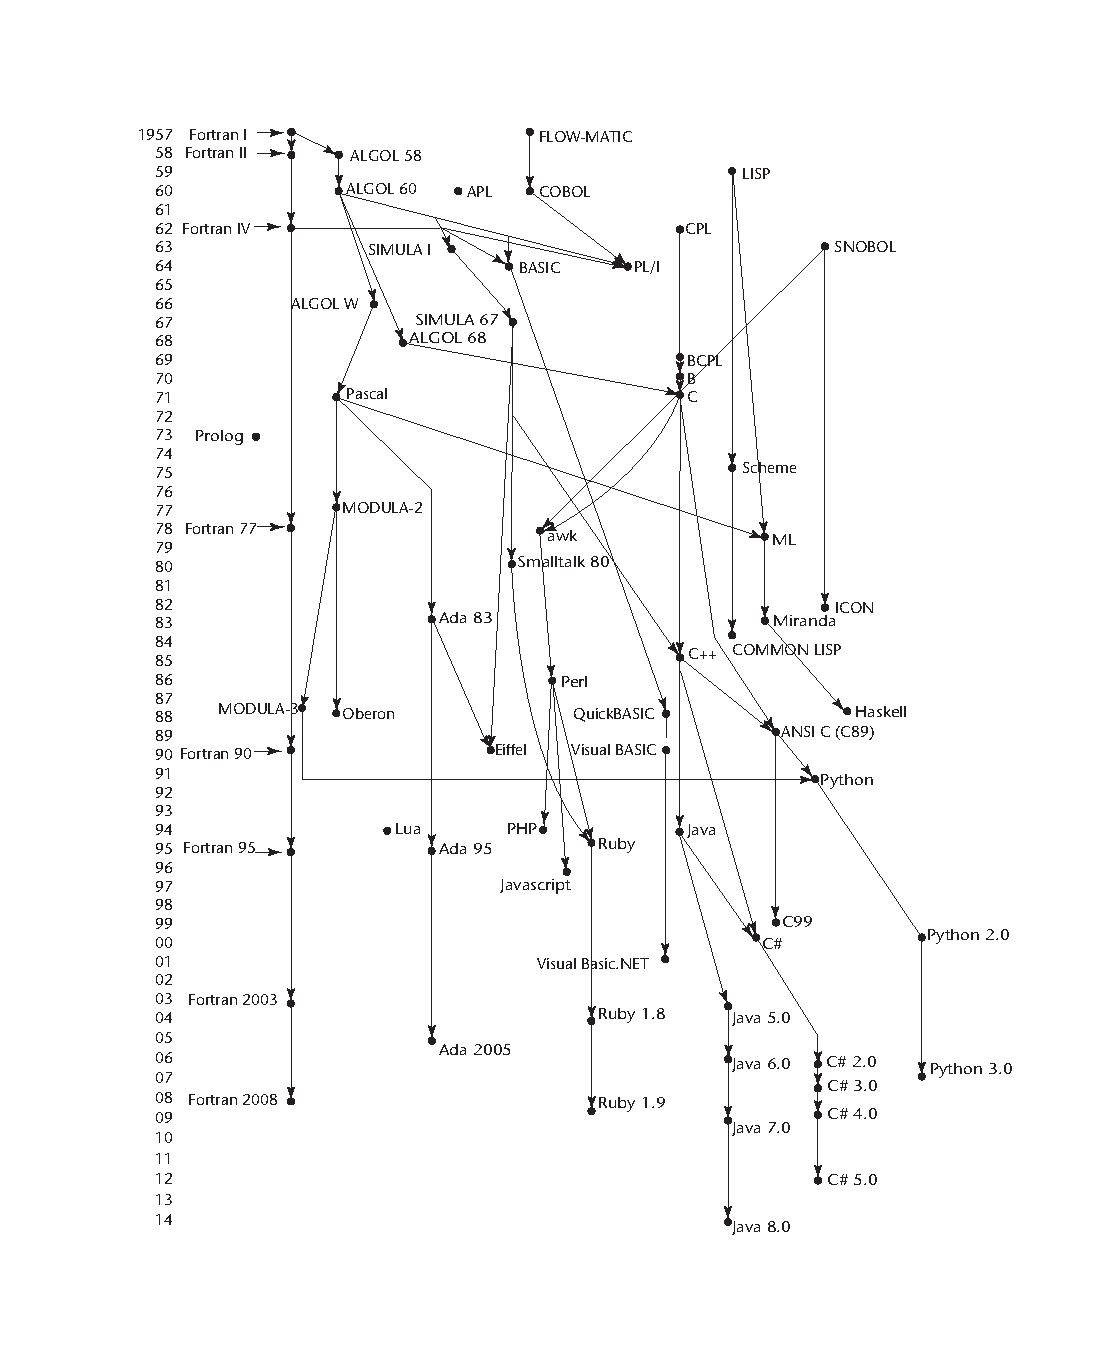
\epsfig{file=figuras/historico,height=.80\textwidth,angle=90}
    \end{center}
\end{frame}


\end{document}


